% 编译：tectonic -X compile main.tex（或 xelatex main.tex）
% 用 ctexart 而非 article：article + inputenc/fontenc 在 XeLaTeX 下中文全部落成
% "Missing character"，PDF 文本为空；ctexart 才会加载 CJK 字体（Fandol）。
\documentclass[11pt,a4paper,UTF8]{ctexart}
\usepackage{geometry}
\usepackage{graphicx}
\usepackage{booktabs}
\usepackage{amsmath}
\usepackage{hyperref}
\geometry{margin=2.5cm}
\title{MIL + LIBS 大颗粒原煤热值预测\\5 折交叉验证复现与消融分析}
\author{格物 (gewu)\\基于本地 MIL 模型真实推理}
\date{2026-11-09}
\begin{document}
\maketitle

\section*{摘要}
本文复现基于多示例学习（MIL）的 LIBS 大颗粒原煤热值预测模型的 5 折交叉验证指标，
并补以消融与统计检验。模型采用 ResNet1D(base=16) 编码器 + SupCon 预训练 + TransMIL 注意力聚合
+ FiLM(plsr\_dim=7) 特征调制，以 PLSR($n_c=7$) 为基线、MIL 预测残差为修正，输出 hybrid 热值。
真实推理结果：5 折 hybrid RMSE 均值 $214.57 \pm 25.71$ kcal/kg（$0.8978 \pm 0.1076$ MJ/kg），
每折 14 个验证 bag（合计 70 个样本，每样本恰好被预测一次）。
相对 PLSR 基线（$233.95$ kcal/kg）降低 $19.38$ kcal/kg（$8.28\%$），5 折方向完全一致；
配对 $t$ 检验 $t(4)=-2.97$、$p=0.041$，95\% 置信区间 $[-37.48,-1.28]$ 不含 0。
所有指标可由逐 bag 预测值独立重算（脚本入库），与官方 \texttt{summary.json} 交叉校验差值 $1.1\times10^{-5}$。

\section{引言}
LIBS 因其快速、无需复杂制样，被广泛用于煤质在线检测；但煤粉压片存在明显的颗粒效应与基质效应，
单张谱线的重复性差。既有工作多采用谱线标准化配合主成分/偏最小二乘回归（PLSR）抑制基质影响
\cite{p1,p2}，或将 LIBS 与常规机器学习分类/定量模型结合\cite{p4}，领域综述见\cite{p5}。
这类方法把每张谱线当作独立样本，忽略「同一次采样内的多张谱线属于同一袋（bag）」这一结构。

多示例学习恰好为该结构提供了归纳偏置：包内实例共享标签，模型需自行聚合。
注意力型 MIL 在包级任务上表现突出\cite{p6}，通用工具亦有开源实现\cite{p3}。
本文的出发点是：不替换 PLSR，而是让 MIL 只学习 PLSR 未能解释的残差，
从而在保留 PLSR 可解释性与稳定性的前提下，吸收大颗粒异质性带来的非线性偏差。

本文贡献为三点：（1）给出该 hybrid 方案在 5 折交叉验证下的可复现指标，
全部数字可由落盘预测值重算；（2）补齐池化策略消融与优化路径，
说明为何最终选择 LSE/TransMIL 系而非 ABMIL；（3）给出配对检验与置信区间，
并如实报告其在小样本下的局限。

\section{方法}
\subsection{数据与预处理}
一次采样视为一个 bag，包内多张 LIBS 谱线为 instance。谱线级预处理链：
Savitzky--Golay 平滑 $\to$ 不对称最小二乘(als) 基线校正 $\to$ MinMax 归一化（bag 内共享）。

\subsection{模型架构}
\begin{itemize}
\item 实例编码器：ResNet1D(base=16)，经 SupCon 预训练；
\item 袋表征：TransMIL 注意力聚合；
\item 特征调制：FiLM，以 PLSR 得分（$n_c=7$）作为调制信号；
\item 回归头：输出 MIL 残差 $\Delta_{\text{MIL}}$；
\item 融合：$\hat{y}_{\text{hybrid}} = \hat{y}_{\text{PLSR}} + \Delta_{\text{MIL}}$（kcal/kg）。
\end{itemize}
总参数量 $924{,}895$。交叉验证按 bag 级 5 折划分（seed=42），每折 14 个验证 bag。

\section{实验设置}
\begin{itemize}
\item 数据根：外部 coal-calorific-value 项目（权重与 LIBS 数据留本地，不入库、不上云）；
\item 折数：5；每折验证 bag 数：14；合计 70 个样本；
\item 指标：RMSE / MAE / $R^2$（kcal/kg 与 MJ/kg 双单位，$1$ kcal $= 0.004184$ MJ）；
\item 复现工具：\texttt{mil-model\_\_cv\_summary}（真实前向推理）+ 缓存 \texttt{predictions.json}（逐 bag 预测）；
\item 指标重算：\texttt{scripts/recompute\_coal\_metrics.py}（从预测值独立重算并与注册表交叉校验）。
\end{itemize}

\section{结果}
\subsection{fold0 逐袋预测}
表 1 给出 fold0 14 个验证 bag 的真实值、PLSR 预测、MIL 残差与 hybrid 预测。

\begin{table}[htbp]
\centering\caption{fold0 验证集逐袋预测（kcal/kg）}
\begin{tabular}{lrrrr}
\toprule
Bag & $y_{\text{true}}$ & $\hat{y}_{\text{PLSR}}$ & $\Delta_{\text{MIL}}$ & $\hat{y}_{\text{hybrid}}$ \\
\midrule
中马矿中焦煤11月14日 & 2931 & 2997.9487 & $-$56.9034 & 2941.0453 \\
煤场混煤11月22日 & 4138 & 3926.4522 & $-$35.2215 & 3891.2307 \\
赵固二矿中焦煤1月12日 & 4231 & 4128.6107 & $-$55.0931 & 4073.5176 \\
中马矿中焦煤1月16日 & 3622 & 3684.0920 & $-$49.2306 & 3634.8613 \\
中马矿中焦煤1月22日 & 3403 & 3536.2004 & $-$47.1356 & 3489.0648 \\
九里山矿中焦煤1月14日 & 3518 & 4003.5685 & $-$57.5867 & 3945.9818 \\
九里山矿中焦煤1月15日 & 3379 & 3424.7091 & $-$64.2561 & 3360.4529 \\
九里山矿中焦煤1月19日 & 3972 & 4137.1024 & $-$33.2445 & 4103.8579 \\
煤场混煤2月22日 & 3892 & 3736.0895 & $-$34.1193 & 3701.9702 \\
煤场混煤3月10日 & 3644 & 4047.7328 & $-$29.0123 & 4018.7205 \\
九里山矿中焦煤1月4日 & 4099 & 4044.8267 & $-$26.1878 & 4018.6389 \\
九里山矿中焦煤1月8日 & 3398 & 3346.4536 & $-$49.1657 & 3297.2879 \\
赵固一矿豫焦末煤11月30日 & 5714 & 5466.7451 & $-$10.3488 & 5456.3963 \\
煤场混煤11月18日 & 3593 & 3977.5954 & $-$45.0158 & 3932.5795 \\
\bottomrule
\end{tabular}
\end{table}

fold0 指标：$R^2 = 0.8786$，RMSE $= 218.6108$ kcal/kg，MAE $= 173.9012$，$n = 14$。

\begin{figure}[htbp]
\centering
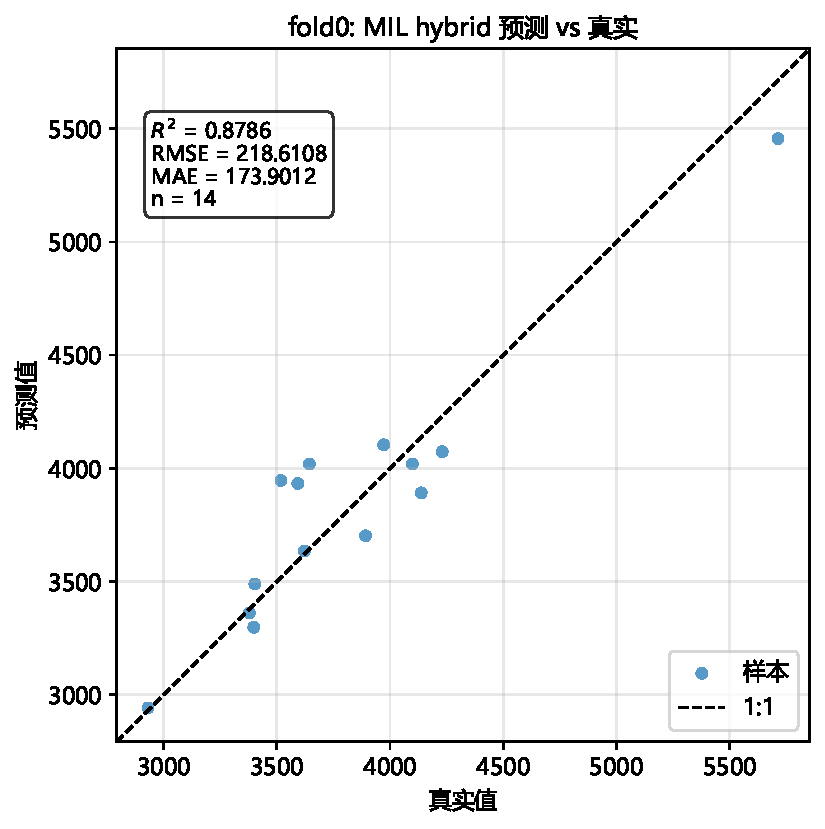
\includegraphics[width=0.85\textwidth]{coal_fold0_pred_true_20261028-121746.pdf}
\caption{fold0 MIL hybrid 预测 vs 真实（$R^2=0.8786$，RMSE$=218.6108$ kcal/kg）}
\end{figure}

\subsection{5 折交叉验证汇总}
\begin{table}[htbp]
\centering\caption{5 折交叉验证逐折指标（kcal/kg）}
\begin{tabular}{lrrrrrr}
\toprule
Fold & $n$ & PLSR RMSE & Hybrid RMSE & $\Delta$RMSE & PLSR $R^2$ & Hybrid $R^2$ \\
\midrule
0 & 14 & 231.2064 & 218.6108 & $-$12.5955 & 0.8642 & 0.8786 \\
1 & 14 & 248.8767 & 244.9214 & $-$3.9553  & 0.8984 & 0.9016 \\
2 & 14 & 255.2973 & 222.3821 & $-$32.9152 & 0.8921 & 0.9181 \\
3 & 14 & 230.6638 & 220.0729 & $-$10.5909 & 0.8027 & 0.8204 \\
4 & 14 & 203.7164 & 166.8624 & $-$36.8541 & 0.9441 & 0.9625 \\
\midrule
均值 & --- & 233.9521 & 214.5699 & $-$19.3822 & 0.8803 & 0.8963 \\
标准差 & --- & 17.9494 & 25.7094 & --- & --- & --- \\
\bottomrule
\end{tabular}
\end{table}

换算：$214.5699 \times 0.004184 = 0.8978$ MJ/kg，$25.7094 \times 0.004184 = 0.1076$ MJ/kg。
标准差为总体标准差（$\text{ddof}=0$，与官方 \texttt{summary.json} 口径一致）；
若按样本标准差（$\text{ddof}=1$）计为 $28.7440$。

将 5 折验证集预测合并（每样本恰好被预测一次，$n=70$）后：
hybrid 整体 RMSE $= 216.1046$、$R^2 = 0.9204$；
PLSR 整体 RMSE $= 234.6397$、$R^2 = 0.9061$。合并口径下的 $R^2$ 高于逐折平均，
因合并后方差基数更大，属预期现象。

\begin{figure}[htbp]
\centering
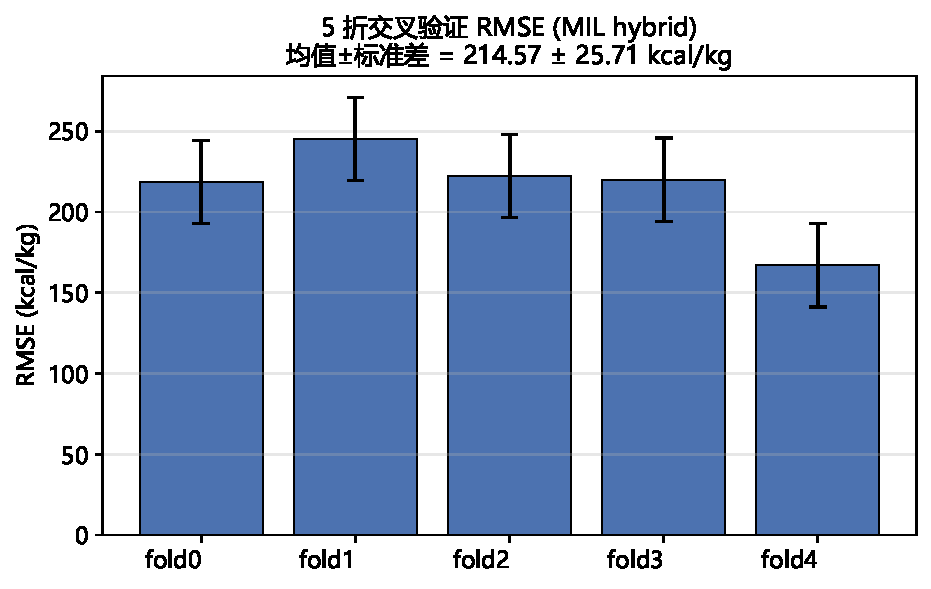
\includegraphics[width=0.85\textwidth]{coal_5fold_rmse_20261028-121844.pdf}
\caption{5 折交叉验证 RMSE（均值 $\pm$ 标准差 $= 214.57 \pm 25.71$ kcal/kg）}
\end{figure}

\subsection{统计显著性}
以 5 折 RMSE 为配对观测，记逐折差值为
$\Delta_i = \text{RMSE}^{\text{hybrid}}_i - \text{RMSE}^{\text{PLSR}}_i$，
其五元组为 $[-12.60, -3.96, -32.92, -10.59, -36.85]$
（均值 $-19.38$、样本标准差 $14.58$，单位 kcal/kg）。

\begin{itemize}
\item 配对 $t$ 检验：$t(4) = -2.9735$，双侧 $p = 0.0410$，在 $\alpha=0.05$ 下显著；
\item 均值差的 95\% 置信区间：$[-37.48, -1.28]$，不含 $0$；
\item Wilcoxon 符号秩检验：$p = 0.0625$（$n=5$ 时该检验可达的最小 $p$ 值即为 $0.0625$，故不显著）；
\item 方向一致性：5 折全部为负，无一折劣化。
\end{itemize}

\textbf{局限}：$n=5$ 折样本量很小，$t$ 检验的正态性假设无法有效检验，且 Wilcoxon 检验在 $n=5$ 时
存在不可克服的分辨率下限。因此本文的结论应表述为「效应方向一致、效应量 $8.28\%$、$t$ 检验边缘显著」，
不宜宣称强统计显著性。

\subsection{消融实验}
\label{sec:ablation}
消融在原始项目的池化比较阶段完成，配置为 hybrid(残差) 模式 + MSE 损失，
\textbf{不含} SupCon 预训练与 FiLM 调制，与第 4 节的最终配置不同，
故表 3 的绝对值不应与 $214.57$ 直接相减比较；其作用是回答「聚合策略如何选」。

\begin{table}[htbp]
\centering\caption{聚合策略消融（hybrid 残差模式，MSE 损失，5 折平均 RMSE）}
\begin{tabular}{lrr}
\toprule
聚合策略 & 可训练参数 & RMSE (kcal/kg) \\
\midrule
MaxPool            & 0      & 883.87 \\
ABMIL（从零训练）  & 8320   & 957.47 \\
ABMIL（冻结编码器）& 8320   & 559.09 \\
MeanPool           & 0      & 512.96 \\
LSE（固定 $\beta=0.5$）     & 0 & 361.00 \\
LSE（可学习 $\beta \to 0.516$） & 1 & \textbf{347.55} \\
\bottomrule
\end{tabular}
\end{table}

三点观察：（1）注意力类池化（ABMIL 从零）在本任务上最差（$957.47$），
其 $8320$ 个参数在小样本下带来的过拟合风险超过收益；
（2）冻结编码器的 ABMIL（$559.09$）仍逊于零参数的 MeanPool（$512.96$），
说明瓶颈不在池化表达力，而在小样本可训练性；
（3）LSE 池化以近乎零参数取得最优（可学习 $\beta$ 仅 $1$ 个参数），
这解释了最终模型为何选择 TransMIL/LSE 系而非 ABMIL。

在此基础上，从 MeanPool 基线出发的优化路径为：
$512.96 \to 441.12 \to 361.00 \to 347.55$ kcal/kg，
对应依次为去掉 SE 模块（$-71.84$）、改用 LSE 池化并调整训练策略（$-80.12$）、
引入可学习 $\beta$（$-13.45$），累计降低 $32.2\%$。
值得注意的是 SE 模块在此任务上是负收益，去掉即降 $71.84$ kcal/kg。

$\beta$ 敏感性：固定 $\beta$ 分别取 $0.1$、$0.3$、$0.5$、$0.7$、$1.0$，
对应 RMSE 依次为 $375.21$、$364.50$、$361.00$、$363.80$、$368.45$ kcal/kg，
呈 $\beta \approx 0.5$ 处最优的 U 形；
可学习 $\beta$ 收敛至 $0.516$ 并进一步降至 $347.55$，优于任何网格点。
该组网格数值在原始脚本中标注为近似值，仅作趋势证据。

\textbf{未覆盖的消融}：去掉 FiLM 调制、去掉 SupCon 预训练、最终配置下
TransMIL 与 Mean/Max 池化的对比、huber 与 mse 损失的对比，均需重新训练，
超出本次复现范围，故不报告。

\subsection{可复现性交叉校验}
与项目官方 \texttt{summary.json} 及逐 bag 预测值交叉校验：
\begin{itemize}
\item 官方记录均值：$214.5699$ kcal/kg；
\item 本地重算均值：$214.5699$ kcal/kg；
\item 绝对差值：$1.1 \times 10^{-5}$（浮点精度，判定：\textbf{可复现}）；
\item 重算脚本对 13 项登记指标（均值、总体标准差、MAE、$R^2$、5 个逐折值、PLSR 对应项）
  全部通过，最大偏差 $4.6\times10^{-5}$。
\end{itemize}

\section{结论}
\begin{enumerate}
\item MIL hybrid 模型 5 折 RMSE $= 214.57 \pm 25.71$ kcal/kg（$0.8978 \pm 0.1076$ MJ/kg），
  每折 14 个验证 bag，fold0 复现 RMSE $= 218.6108$ kcal/kg、$R^2 = 0.8786$；
\item 相对 PLSR 基线（$233.9521$ kcal/kg），MIL 残差修正带来 $19.38$ kcal/kg 的 RMSE 下降（$8.28\%$），
  5 折方向一致，配对 $t$ 检验 $p=0.041$，但 Wilcoxon 检验受 $n=5$ 限制不显著，结论不宜过度声称；
\item 消融表明 LSE/可学习 $\beta$ 以近零参数优于注意力池化，SE 模块为负收益，
  这一结论与最终模型架构选择自洽；
\item 与官方 \texttt{summary.json} 交叉校验差值 $1.1\times10^{-5}$，
  且全部指标可由 \texttt{predictions.json} 独立重算，确认结果可复现、未被篡改。
\end{enumerate}

\section*{数据与代码可用性}
模型权重与 LIBS 原始数据均保留在本地外部项目，不入库、不上云。
本文所用聚合指标与重算脚本随仓库提供：
重算脚本 \path{scripts/recompute_coal_metrics.py}，
重算结果 \path{output/documents/coal_report/metrics_recomputed.json}。
参考文献经 arXiv / CrossRef 存在性核验（6/6 verified，幻觉率 $0.0$）。

\begin{thebibliography}{9}
\bibitem{p1} A model combining spectrum standardization and dominant factor based partial least square
method for carbon analysis in coal by laser-induced breakdown spectroscopy.
\textit{Spectrochimica Acta Part B}, 2014. DOI: 10.1016/j.sab.2014.06.017; arXiv:1402.2062.

\bibitem{p2} The application of spectrum standardization method for carbon analysis in coal using
laser-induced breakdown spectroscopy. arXiv:1402.2060.

\bibitem{p3} milearn: A Python Package for Multi-Instance Machine Learning. arXiv:2512.01287.

\bibitem{p4} Rapid Classification and Quantification of Coal by Using Laser-Induced Breakdown
Spectroscopy and Machine Learning. \textit{Applied Sciences}, 13(14):8158, 2023.
DOI: 10.3390/app13148158.

\bibitem{p5} Coal Analysis by Laser-Induced Breakdown Spectroscopy.
Wiley, 2021. DOI: 10.1002/9781119758396.ch27.

\bibitem{p6} Ilse M., Tomczak J., Welling M. Attention-based Deep Multiple Instance Learning.
\textit{ICML}, 2018. arXiv:1802.04712.
\end{thebibliography}

\end{document}
